\documentclass[12pt]{article}

\usepackage{tgtermes}
\usepackage{epsf}
\usepackage{epstopdf}
\usepackage{amsmath}
\usepackage{graphicx}
\usepackage{booktabs}
\usepackage[colorlinks=true,linkcolor=blue,citecolor=blue]{hyperref}
\usepackage{dcolumn}
\usepackage{amsmath, amsthm, amssymb}
\usepackage{mwe}
\usepackage{url}
%\usepackage{harvard}
\usepackage{fancyheadings}
\usepackage{longtable}
\usepackage{authblk}
\usepackage{setspace}
%\usepackage[nomarkers]{endfloat}
\usepackage{float}
\usepackage{bbm}
%\usepackage{titling}
\usepackage{subcaption}
\usepackage{algorithm}
\usepackage{algorithmic}
\usepackage{import}
\usepackage[backend=biber,style=authoryear,
sorting=ynt,citestyle=authoryear]{biblatex}
\addbibresource{papercitations.bib}
%\usepackage[nomarkers,nofiglist,notablist]{endfloat}
\usepackage{subcaption}
\usepackage{caption}

\onehalfspacing
\textwidth 6.5in \oddsidemargin 0in \evensidemargin -0.6in
\textheight 8.5in \topmargin -0.2in

\newcolumntype{L}[1]{>{\raggedright\let\newline\\
		\arraybackslash\hspace{0pt}}m{#1}}
\newcolumntype{C}[1]{>{\centering\let\newline\\
		\arraybackslash\hspace{0pt}}m{#1}}
\newcolumntype{R}[1]{>{\raggedleft\let\newline\\
		\arraybackslash\hspace{0pt}}m{#1}}
\newcolumntype{P}[1]{>{\raggedright\tabularxbackslash}p{#1}}

\newtheorem{theorem}{Theorem}[section]
\newtheorem{corollary}[theorem]{Corollary}
\newtheorem{proposition}[theorem]{Proposition}
\newtheorem{lemma}[theorem]{Lemma}

\captionsetup{justification=centering,singlelinecheck=false}


\newcommand{\xsub}[1]{%
	\mbox{\scriptsize\begin{tabular}{@{}c@{}}#1\end{tabular}}%
}

%\renewcommand{\thetable}{\Roman{table}}

\begin{document}
	
	
	
	
	\linespread{1.2}\title{\vspace{-0.5in} Does Hospital Leadership Matter?\\ \large Evidence from Pay-for-Performance Incentives} 
	
	\date{\today}
	
	\author{\vspace{10mm}Hanna Glenn\footnote{Department of Economics, Emory University, 1602 Fishburne Drive, Atlanta, GA 30322, hanna.glenn@emory.edu.} }
	
	\maketitle
	%\setlength{\droptitle}{-10pt}
	
	\vspace{-0.2in}
	
	\singlespacing\maketitle


 \vspace{3mm}
	
    \begin{abstract}
		{\small
        In many industries, not-for-profits (NFP) make up the majority of firms in the market. Understanding the objectives of these firms is important as they respond to incentives, but NFP firms have underlying goals that make understanding their objectives difficult. For hospitals in particular, there is mixed evidence on whether NFP hospitals differ meaningfully from for-profit (FP) hospitals. In this paper, I investigate whether leadership team composition of NFP hospitals affects how similarly they behave to for-profits. I use a novel data set on NFP hospital executives in the US (2009-2015) to investigate whether the presence of clinically trained executives affects hospital behavior. In particular, I leverage two pay-for-performance initiatives in the US enacted in 2012, and measure the  readmission and mortality rate responses between FP, NFP, and NFP with and without clinically trained executives. I find that NFPs without clinically trained executives behave more like FPs than other NFPs. This is consistent with theoretical predictions under the assumption that NFP hospitals with clinically trained executives value societal outcomes more than those without clinically trained executives.
		} 
	\end{abstract}
	
	
	
	
	\vspace{0.8in}
	
	\noindent Keywords: 
	
	\noindent JEL Codes: 
	
	\onehalfspacing
	
	\newpage

  The objectives and behaviors of firms that are not classic for-profits are not easily determined, and an extensive literature has sought to understand these types of firms. Not-for-profits (NFP) are thought to gain utility not solely from monetary profit, but also through accomplishing societal benefit. Researchers have speculated a variety of objective functions that could motivate NFP firms such as maximizing prestige, income, or a quality/quantity trade-off (\cite{steinberg1986revealed}). Empirical contributions to this literature center around investigating behaviors that differ between for-profit (FP), private NFP, and government firms (\cite{sloan2000not}). In this paper, I investigate whether differences in observed behavior between for-profit and not-for-profit hospitals vary differentially by leadership team composition. 
  
  Hospitals have been a common focus when seeking to understand NFP firms. This is because, first, there are different hospital ownership types within the industry, giving researchers the ability to compare the behaviors of NFPs and FPs. Second, private NFP hospitals make up 50\% of all hospitals in the US, and staff, on average, 207 beds. For comparison, FPs make up around 36\% of hospitals and staff 107 beds (\cite{ASPE_2023}). Thus, NFP behavior in the hospital industry is relevant, and directly affects consumers of health care. However, it remains unclear what objective function drives NFP hospital behavior, and whether NFP hospitals are meaningfully different from FP hospitals (\cite{sloan2000not}; \cite{erus2002inferring}; \cite{deneffe2002not}; \cite{horwitz2009hospital}). 
  
  While the characterization of being for-profit or not-for-profit is certainly important, there could be other characteristics that affect hospital behavior that are not perfectly correlated with individual ownership status. Researchers have focused in particular on explaining the differences in NFP behavior by the market they exist again (citations). I argue that an observable and economically meaningful factor is the composition of leadership teams. Firm leadership varies widely across firms and potentially drives differences in objectives even within NFPs. In large, publicly traded firms, executive characteristics are shown to be correlated with firm performance, indicating that there is more to firm behavior than ownership status (\cite{bertrand2003managing}; \cite{matsa2013female}; \cite{ahern2012changing}). If hospital objectives differ in how they value monetary profit vs. gains to society, then ownership status certainly plays a role in these valuations, but the question remains as to whether management also plays an important role. I contribute to our understanding of hospital and NFP behaviors by investigating whether occupational background, specifically clinical training in executives, affects hospital response to pay-for-performance incentives.

  Using publicly available tax forms, I construct a novel data set of NFP hospital executives from 2009-2015. I link hospitals in this data to characteristics in the American Hospital Association (AHA) survey and Hospital Compare data. I leverage various pay-for-performance initiatives in 2012 to investigate differential hospital responses between for-profits, NFPs without clinically trained executives, and NFPs with clinically trained executives. 
  
  I estimate how the interaction between hospital type and post program enactment affects readmission and mortality rates among different groups. Under the assumption that hospitals would have continued to behave similarly in the absence of the programs, and that leadership teams do not change endogenously with the programs, I identify the differential response to pay-for-performance incentives by different hospital types. Among the hospitals in the data, hospitals with clinically trained executives are the minority, and differ on average from other hospitals along various dimensions. Thus, my preferred specification is synthetic difference-in-differences, to analyze a group of comparison hospitals with similar characteristics to treatment hospitals.\footnote{I also present results for the full sample, and find qualitatively similar results.} 
  
   While all hospital types decrease readmission rates after the programs are enacted, for-profits and not-for-profits without clinically trained executives decrease readmissions more than not-for-profits with clinically trained executives. That is, NFPs without clinically trained executives respond to incentives more similarly to FPs than other NFPs. I then consider whether this effect is due to clinically trained executives being a signal of underlying hospital preferences, or changing hospital preferences in a way that then affects behavior. I decompose the two by leveraging hospitals who change their propensity to hire a clinically trained executive at some point in the sample, which I find is not occurring endogenously with the change in incentives. The results of this analysis suggest that the difference in response is driven by changing hospital preferences, not as a signal of underlying preferences. While readmissions and mortality were targeted directly by the programs, I also consider uncompensated care and case mix index as outcomes, since re-allocation of resources and patient selectivity are potential mechanisms to changing hospital outcomes. (results of this analysis here)

    This paper contributes to three strands of literature. First, it adds to our understanding of what underlies NFP hospital behavior. There is mixed evidence on whether NFP behavior differs from FP behavior: costs, uncompensated care, technology adoption, and quality (\cite{sloan2000not}; \cite{eggleston2008hospital}; \cite{moscelli2018effect}; \cite{moscone2020public}). Underlying hospital are hospital objectives. To this point, researchers have found that NFPs do not act as purely profit maximizers, but maximize some combination of profit and output (\cite{deneffe2002not}, \cite{chang2011not-for-profit}). A paper with an approach similar to mine which investigates hospital behavior is \citeauthor{chang2011not-for-profit} (\citeyear{chang2011not-for-profit}), which looks at the effect of a cost shock on likelihood of shutting down and mix of profitable services. They find that NFPs and FPs are equally as likely to shut down after the shock, but only NFPs adjust their mix of profitable services. Similarly, I investigate a change in incentives to hospitals, but I look at the differential impacts of leadership teams within not-for-profits. This paper adds to our understanding of inputs into not-for-profit hospital objective functions. 

    Second, many researchers have documented a correlation between executive backgrounds, specifically for CEOs, and firm performance, starting with \citeauthor{bertrand2003managing} (\citeyear{bertrand2003managing}), who show that manager fixed effects are an important driver of many firm behaviors and decisions. Female board members are associated with better oversight and more women executives (\cite{matsa2011chipping}; \cite{adams2009women}), but are negatively correlated with firm value (\cite{ahern2012changing}). Having more female executives is correlated with female employee wages and corporate strategies (\cite{flabbi2019female}; \cite{matsa2013female}); young male CEOs tend to be more aggressive in mergers and acquisitions, while those with military experience are less aggressive (\cite{levi2010deal}; \cite{benmelech2015military}); CEOs with general ability tend to receive higher pay and perform better (\cite{kaplan2012ceo}; \cite{custodio2013generalists}; \cite{adams2018director}; \cite{frydman2019rising}). Further, Chief Diversity Officers are not found to have any effect on hiring more diversely in universities (\cite{bradley2022impact}). 
    
    Due to data limitations, many of these studies focus on large, publicly traded firms in the US. \citeauthor{brickley2010board} (\citeyear{brickley2010board}) has the only study to my knowledge answering this question in the US NFP context. Using exogenous variation in expected Medicare profits, the authors find that having an internal board of directors increases CEO compensation, and having physician board members decreases public donations (\cite{brickley2010board}). Additionally, two studies focus on hospital performance in other countries. \citeauthor{janke2019impact} (\citeyear{janke2019impact}) uses data from England to study whether CEOs affect hospital production, and find no association (\cite{janke2019impact}). However, \citeauthor{otero2022managers} (\citeyear{otero2022managers}) investigates the role of CEOs in public hospitals and Chile, and finds an 8\% decrease in mortality rates for hospitals with top managers (\cite{otero2022managers}). I contribute to this literature by considering the executive team as a whole rather than just CEOs, by investigating a context which is not largely studied but is policy relevant, NFP US hospitals, and by leveraging a unique executive characteristic pertinent to that context. 

    Finally, I contribute to our understanding of how providers respond to pay-for-performance incentives in health care. The most in depth study of how hospitals respond to HRRP is \citeauthor{gupta2021impacts} (\citeyear{gupta2021impacts}), who finds that hospitals decreased readmissions by 5\% and mortality rates by 2\% on average as a result of the program, confirming prior studies (\cite{mellor2017does}; \cite{ziedan2018essays}; \cite{ody2019decreases}; \cite{gupta2021impacts}). Around 40\% of the decrease in readmissions is due to selective patient practices. Research on HVBP generally finds that the program had no effect on underlying hospital quality (\cite{us2015hospital}; \cite{norton2018moneyball}; \cite{friedson2019so}). This paper contributes to our understanding of how characteristics of hospitals affect response to pay-for-performance incentives. 

    

    \section{Setting}

    \subsection{Not-for-Profit Hospital Leadership}

    Not-for-profit firms differ from for-profits mainly in that for-profit firms distribute revenue to stakeholders, while not-for-profits reinvest profit back into the firm. Another important distinction is that NFPs are, in general, driven by a mission to better society. Additionally, NFPs in the US receive tax benefits for this designation. 
    
    NFPs are governed by a board of directors, whose role is to set broad goals and strategies, and provide general oversight. The board selects executives, the highest level of management of a firm, to carry out day-to-day operations. An executive team usually consists of at least a CEO and CFO, but every NFP is different in exactly how they structure their executive team. Many hospital executives specialize in health care settings by getting degree(s) in health care management, or an MBA specific to health care. There are specific positions that are often filled by someone with clinical training, such as a Chief Medical Officer, and doctors can even find themselves in other top managerial positions as well, such as CEO or president. While some doctors earn additional degrees before stepping into an executive role, this is not a necessary condition to becoming a physician executive. 

    Anecdotal evidence is mixed on the benefits of hiring physician executives. On one hand, physicians bring a unique combination of clinical expertise and being comfortable with administration, and they can bring insights that improve hospital outcomes (\cite{Stajduhar_2023}, \cite{Ahmed_2022}). Alternatively, physicians may not always be adequately trained to enter into high level management positions, and therefore are not equipped to lead a firm (\cite{HarvardBusinessReview2018}). 

    All tax-exempt organizations in the US are required to file a Form 990 with Internal Revenue Services (IRS) each year. There are different types of forms, but any organization grossing over \$200,000 must file the most extensive Form 990. Sections of this form include a statement of revenue, statement of functional expenses, a balance sheet, and, as used in this project, a list of all key employees, executives, and board members. Each firm is required to report the name and title, average hours per week, position, and compensation of their board members and executive leaders. 

  
    \subsection{Pay-for-Performance Policies}\label{sec:hrrp}

    Two programs were passed as part of the Affordable Care Act that focused on pay-for-performance incentives for hospitals, the Hospital Readmissions Reduction Program (HRRP), and the Hospital Value Based Purchasing Program (HVBP). The HRRP focused on penalizing hospitals with poor quality in terms of readmission rates, and the HVBP fpcused on rewarding hospitals with high quality in terms of something. 

    In October 2011, the Center for Medicare and Medicaid Services (CMS) released a set of rules under HRRP that mandated penalties for hospitals with above average readmission rates. A readmission is when a patient returns to the hospital within 30 days of being discharged from a previous stay; avoidable readmissions are a bad outcome for patients and increase health care spending. The goal of HRRP is to lower readmissions through better care coordination, less initial stay complications, and better post-care instructions. Beginning in October 2012, hospitals with higher readmission rates than the national average in pneumonia, heart failure, or AMI (after adjusting for demographic characteristics) receive a fixed lower reimbursement rate for all Medicare patients seen in their hospital. In 2015, CMS also included chronic obstructive pulmonary disease, coronary artery bypass graft surgery, and elective primary total hip arthroplasty and/or total knee arthroplasty as conditions which go into the penalty calculation (\cite{CMS}). 
    
    Penalized hospitals pay penalties in the form of a fixed rate for every Medicare patient regardless of the condition. The rate began at 1\% and increased to 3\% in 2015. Further, CMS does not distinguish a necessary readmission from an avoidable readmission; any repeat hospital visit is included in the penalty calculation. Excess readmission rates are calculated using a rolling look-back period of 3 years to determine whether the hospital is penalized. Therefore, hospitals had incentive to react immediately once details of the program were announced in October of 2011. These penalties are not insignificant; penalized hospitals paid, on average, 4-5\% of revenue. 

    The HVBP Program instead rewards hospitals with high quality or shown improvement in quality. Specifically, CMS deducts Medicare payments by 2\%, collects this sum, and divides it among the rewarded hospitals. Several quality and cost measures in categories safety, efficiency and cost reductions, clinical outcomes, and community engagement, are combined to create a single score metric for each hospital. Hospitals are then compared to each other and score points for being above average quality and for showing improvement (\cite{CMS_2023}). 

    

	\section{Data}\label{sec:data}

    Hospital executive teams are understudied partly because of the inaccessibility of granular information. I construct a novel data set of not-for-profit hospitals in the US that contains names, titles, and positions of all board members and executives tied to the hospital from 2009-2015. I gather this data from publicly available Tax Form 990s, which every sufficiently large not-for-profit files each year in the US. To my knowledge, this is the first large scale gathering of executive names from these forms.\footnote{\citeauthor{brickley2010board} (\citeyear{brickley2010board}) collects compensation information for a select number of hospitals.} 

    The historical tax forms for all not-for-profits are housed by ProPublica.\footnote{https://projects.propublica.org/not-for-profits/} I use the NonProfit Explorer API to extract Employee Identification Numbers (EIN) of not-for-profits classified as a hospital according to their National Taxonomy of Exempt Entities (NTEE) code. After filtering out associations and specialty hospitals, there are approximately 3,000 not-for-profit EINs. Importantly, linking EINs to other hospital information is crucial for the analysis. I rely on matching by location and name of hospital in the tax forms and AHA data. I confidently match 1200 EINs to an AHA identification number based on exact name matches within the same state. I compare the matched hospitals to non-matched hospitals in Appendix \ref{app:matched}.
    
    For each of the 1200 EINs, I then extract web URLs to Form 990 PDFs in each year. I download these locally and use optical character recognition (OCR) text extraction methods to scrape the relevant section of the PDF, which is titled ``Officers, Directors, Trustees, Key Employees, and Highest Compensated Employees". Finally, I use string cleaning methods to identify names and positions for each EIN, year. I also identify titles indicating clinical training: MD, Dr., or DO. Using OCR extraction can be unreliable in some instances if the text is handwritten or small. Therefore, I manually record names, positions, and titles for observations that are missing after the initial extraction. This yields 852 not-for-profit hospitals that are matched to AHA data, and are not missing text information. 

    Due to the lack of consistency in the organization of executive teams, I focus mainly on the executive teams as a whole instead of specific positions. I drop anyone who is solely a board member, and focus on those who have executive in their title or are labeled as a president or vice president of a department. I create various hospital-level characterizations based on their executive teams, such as the existence of a clinically trained executive, the number of clinically trained executives, the number of total executives, and whether the hospital has a Chief Medical Officer. Summary statistics for these variables are shown in Table \ref{leader_sumstats}.

    \import{Tables}{leader_sumstats.tex}

    I merge the created sample of not-for-profits with all for-profits in the AHA survey. The outcomes I consider are readmission and mortality rates, which are directly targeted in the pay-for-performance policies, and are from the CMS Hospital Compare data. I combine readmission and mortality rates for pneumonia, AMI, and heart failure (the relevant HRRP conditions) into a weighted average based on the number of patients in each condition. Additionally, I include several relevant hospital characteristics. Number of beds, whether the hospital is an academic medical center, is physician owned or is system affiliated, all come from the AHA survey. Uncompensated care comes from HCRIS, and case mix index, which measures patient complexity, comes from CMS. Whether the hospital was penalized under HRRP or received payments under HVBP is found in the HCRIS data. Finally, I limit to years 2010-2014.

    % In Table \ref{sumstats}, I present summary statistics for hospital variables. There are 3,766 total hospitals in the sample, with 150 beds on average. Hospitals in the sample are less likely to be penalized for AMI than either heart failure or pneumonia under the HRRP program. On average, 20\% of patients with one of these conditions would be readmitted. While readmission rates for the specific conditions are similar, the highest likelihood of readmission is for heart failure patients. Alternatively, AMI is the most dangerous condition in terms of mortality rates. 

    %\import{Tables}{overall_sumstats.tex}

    I present a table of means for each hospital type (for-profit, in-sample not-for-profits, and not-for-profits with and without a clinically trained executive) in Table \ref{tab:sumstats_samples}. Slightly over half of the hospitals are classified as not-for-profit with leadership information. There are key differences in not-for-profits with and without clinically trained executives: those with MDs are larger, more likely to be penalized, have higher uncompensated care, and more complex patients. I discuss the implications of these differences for identification in Section \ref{sec:model}. 

    \import{Tables}{sample_sumstats.tex}

    I plot patient-complexity adjusted readmission and mortality rates across time for different hospital types in Figure \ref{fig:weighted_read_mort_graph}. For-profit hospitals have the highest readmission rates prior to 2012. While the trend in readmission rates behaves similarly across hospital types prior to the programs taking affect, there are differential trends after the programs. NFPs without cilnically trained executives decrease readmissions more similarly to FPs than other NFPs. In mortality rates, NFPs with a clinically trained executive have the lowest rates before the programs, but differentially continue with an increasing trend in mortality after the programs. While this is purely descriptive evidence, the trends in outcomes point to more similar behavior between for-profits and NFPs without clinically trained executives in comparison to NFPs with a clinically trained executive.

    \begin{figure}[ht!]
    \centering
        \caption{Outcomes Over Time}
        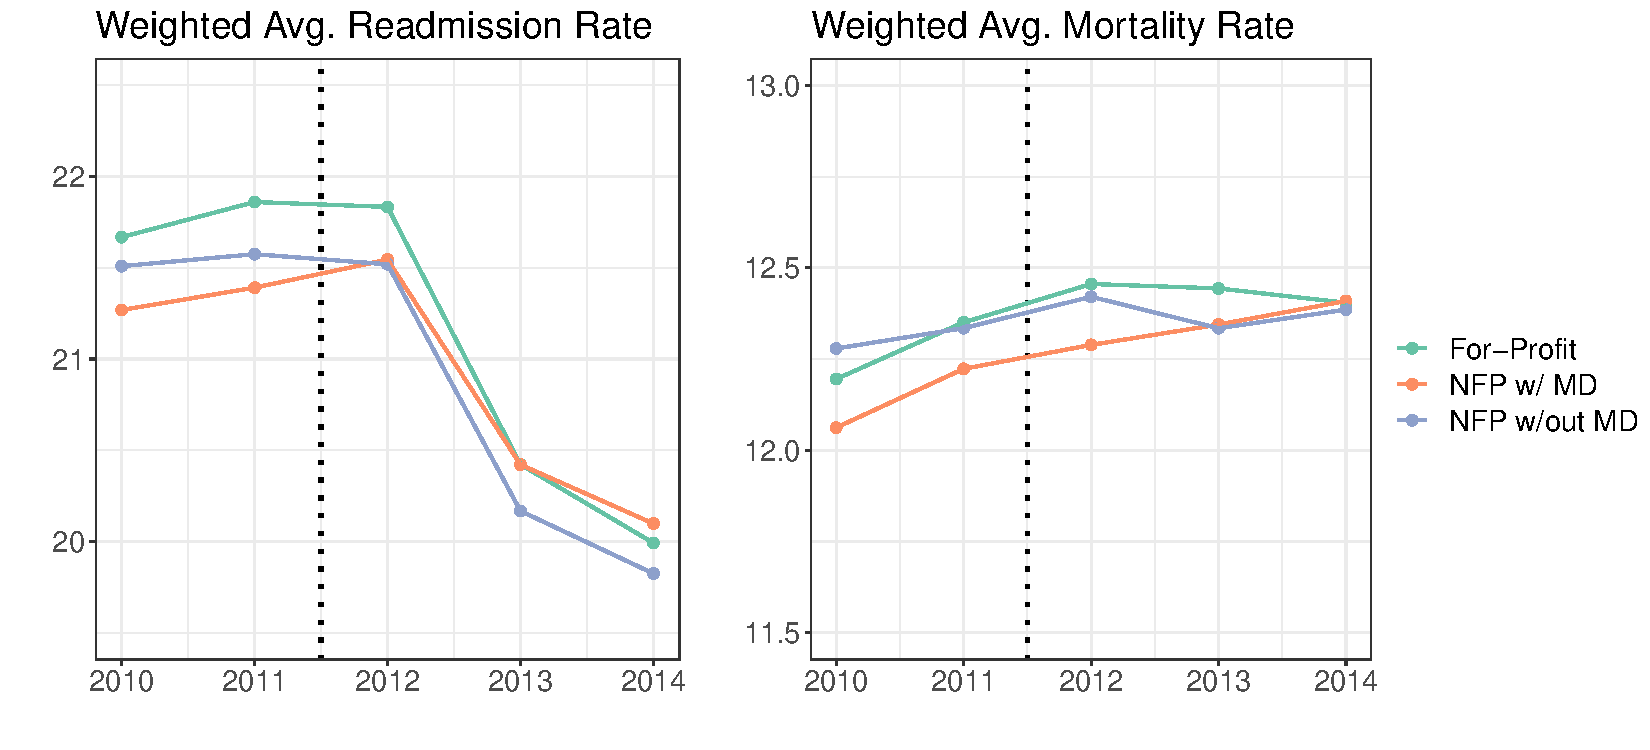
\includegraphics[width=\textwidth]{Objects/weighted_read_mort_adjusted_graph.pdf}
        \label{fig:weighted_read_mort_graph}
    \end{figure}


    \section{Model and Empirical Strategy}\label{sec:model}

    I model hospital behavior in two simplified scenarios: where quality does not directly affect profit, and where it does. Pay-for-performance incentives essentially incorporate performance directly into a hospital's profit function. Here, I think of performance as quality of care, which is inversely related to readmission and mortality rates. While the literature speculates about the true form of NFP objective functions, we can generally think of hospitals choosing some linear combination of profit and societal benefit. Intuitively, a hospital that places more weight on profit (for-profit type) will only care about quality when it enters into the profit function, and therefore will respond more drastically to quality entering the profit function than a hospital who already cared about quality before the incentives. Therefore, hospital response to pay-for-performance incentives reveals something about their underlying preference on profit vs. societal outcomes. 

    Formally, I model the hospital objective function as a weighted average of profit and societal (or patient) outcomes. For simplicity, I abstract away from quality having a direct effect of quantity and price, which does not drastically change the main results. Without any financial incentives to increase quality, hospital quality is decided by:  
    
    $$\max_{\theta}\hspace{2mm}\alpha\left[R - c_{\theta}(\theta) \right] + (1-\alpha) u(\theta),$$

    \noindent where $R$ is net revenue, $c_{\theta}(.)$ is an increasing cost function specific to quality $\theta$, $u(.)$ is extra utility gained from quality, which is increasing and concave in $\theta$, and $\alpha\in[0,1]$ captures how much the hospital cares about profit vs. societal benefit. There is an implicit stay open condition throughout the model. Taking the first order condition yields 

    $$(1-\alpha)u'(\theta) = \alpha c_{\theta}'(\theta),$$

    \noindent marginal benefit equals marginal cost of increasing quality. Solving for $u'(\theta)$ and differentiating with respect to $\alpha$ yields

    $$\frac{du'(\theta)}{d\alpha} = \frac{1}{(1-\alpha)^2}c_{\theta}'(\theta) > 0.$$

    \noindent Thus, by the Implicit Function Theorem, 

    $$\frac{d\theta}{d\alpha} = \frac{du'(\theta)/d\alpha}{du'(\theta)/d\theta} < 0.$$

    \noindent That is, the more weight on profit, the lower quality of care chosen by the hospital.

    In a world with pay-for-performance incentives, which can either look like benefits from high quality (such as HVBP) or penalties for low quality (as in HRRP), quality directly affects revenue. Thus, $R(\theta)$ is an increasing function of $\theta$, and I assume that the marginal financial benefit of increasing quality is greater than the marginal cost ($R'(\theta)\geq c_{\theta}'(\theta))$. Thus, the new first order condition yields:

    $$u'(\theta) = \frac{\alpha}{1-\alpha} \left[c_{\theta}'(\theta)-R(\theta)\right] \leq 0.$$

    \noindent Taking the derivative of this with respect to $\alpha$,

    $$\frac{du'(\theta)}{d\alpha} = \frac{1}{(1-\alpha)^2}c_{\theta}'(\theta).$$

    Thus,

    $$\frac{d\theta}{d\alpha} = \frac{du'(\theta)/d\alpha}{du'(\theta)/d\theta}\geq0.$$

    Therefore, in a world with financial incentives on quality, quality is increasing with more weight placed on profit. The purpose of this paper is to investigate the response of hospitals with different $\alpha$ when a policy changes hospital incentives using pay-for-performance. Hence, I combine the results found in each scenario into one response function that depends on $\alpha$, where $\theta_2$ is quality under pay-for-performance incentives and $\theta_1$ is quality with no financial incentive to quality. Thus,

    \begin{align*}
        \frac{d\Delta\theta}{d\alpha}&=\frac{d(\theta_2-\theta_1)}{d\alpha}\\
        &=\frac{d\theta_2}{d\alpha}-\frac{d\theta_1}{d\alpha}\\
        &\geq 0.
    \end{align*}


    The theoretical prediction is that change in quality depends on how much weight the hospital places on profit vs. societal benefit. Particularly, hospitals with more weight on profit respond more than hospitals with more weight placed on societal benefit. In reality, $\alpha$ is not revealed by the hospital, except in the case of for-profits, who have revealed that they have a high $\alpha$ by their ownership status. However, not-for-profit behavior on average does not bring much clarity about their objectives. An observable and economically relevant characteristic of a hospital that could affect $\alpha$ is composition of their leadership team. Thus, I compare the response to incentive change between for-profits and not-for-profits with different leadership teams to bring clarity on how this might point to underlying $\alpha$.
    

    \subsection{Estimation}

    In light of the theoretical predictions, I first test empirically whether different sub-samples of not-for-profits respond to program incentives differently than for-profits. I estimate the following regression equation:

    \begin{equation}
    \label{eq:forprofit}
    y_{ht} = \beta (\text{For-Profit}_h \times \text{Post Programs}_t) + \gamma_{h} + \delta_t + \epsilon_{ht}
    \end{equation}

    \noindent where $y_{ht}$ is one of the outcome variables discussed in Section \ref{sec:data}, $\beta$ is the coefficient of interest capturing the effect of being for-profit after the programs were introduced, and $\gamma_h$ and $\delta_t$ are hospital and time fixed effects, respectively. For each outcome, I estimate three models with differing comparison groups: all NFPs, NFPs with a clinically trained executive, and NFPs without a clinically trained executive. I also directly estimate the difference in response of NFPs with and without a clinically trained executive:

    \begin{equation}
    \label{eq:clinical}
    y_{ht} = \beta (\text{No MD Exec}_h \times \text{Post Programs}_t) + \gamma_{h} + \delta_t + \epsilon_{ht}
    \end{equation}

    An important distinction is whether the classification of NFPs by leadership team is time-varying. For overall ownership status, switching is rare, and I limit to those who never switch. However, hospital executive teams are dynamic, and whether or not a hospital employs a clinically trained executive in each period may change. Therefore, for simplicity, I first present effects of having a clinically trained executive among stable executive teams, i.e., NFPs with no change in their propensity to hire a clinically trained executive. 

    Additionally, under certain assumptions that I discuss in Section \ref{sec:identification}, using executive team changes can be advantageous in better understanding underlying hospital motives. There are two mechanisms to having a clinically trained executives affecting outcomes: first, a clinically trained executive could be a signal of the underlying weight placed on profit, $\alpha$. Second, hiring a clinically trained executive who carries out day-to-day operations in a distinct way effectively changes $\alpha$. Thus, I use two types of variation in clinically trained executives to disentangle the two: a variable for whether the hospital ever hires a clinically trained executive, and a variable for whether the hospital has a clinically trained executive in 2012 when the programs took place. I use the same empirical specification with these two variables as the independent variation in executive teams, and limit the sample to the relevant comparison group: 

    \begin{equation}
    \label{eq:decomp}
    y_{ht} = \beta (\text{Never/No 2012 Exec}_h \times \text{Post Programs}_t) + \gamma_{h} + \delta_t + \epsilon_{ht}
    \end{equation}

    \subsection{Identification}\label{sec:identification}

    To identify the causal effect of hospital type on hospital program response, I rely on several assumptions. First, I assume that, absent the program enactments, different hospital types would have had parallel trends in outcomes. While I see no evidence of pre-trends, Table \ref{tab:sumstats_samples} does show that hospitals with a clinically trained executive are different than other hospitals in multiple characteristics. Therefore, there may be concern that there are systematic differences between hospital types that could be driving the results. Therefore, my main specification uses the synthetic difference-in-differences method established in \citeauthor{arkhangelsky2021synthetic} (\citeyear{arkhangelsky2021synthetic}). This method creates unit weights that more heavily count comparison hospitals that have similar trends in outcomes prior to the programs. It also weighs time periods that balance pre-program with post-program for the comparison hospitals. Then, a simple two way fixed effects estimator is used with these weights. This is a more robust average treatment effect that relies less on a strong parallel trends assumption (\cite{arkhangelsky2021synthetic}). I present the synthetic diff-in-diff estimates as the main results, and they are largely similar to the standard two way fixed effects results in Appendix \ref{app:fullsample}. Further, while ultimately I employ a synthetic difference-in-differences method, the conceptual identification is identical to a standard difference-in-differences.

     Second, I assume that executive teams are not determined endogenously with the programs. In the main specification, I limit to executive teams which do not change their propensity to hire an MD over time. Thus, I rely on this assumption so that I am not conditioning on an outcome. In supplementary analyses, I use executive team changes to disentangle signalling vs. managing effects, which is only identified if leadership changes are uncorrelated with the policies. 

     I assess the validity of this assumption in two ways. First, I analyze whether changes in clinically trained executives are concentrated around the enactment of both HRRP and HVBP, 2011-2012. Second, I analyze whether hospitals who end up getting penalized through HRRP are more likely to change clinically trained executives on their team than non-penalized hospitals, and similarly for hospitals who end up getting extra payments for high quality of care through HVBP. That is, are hospitals that expect to be affected by the programs more likely to hire or fire clinically trained executives? I consider changes along having any clinically trained executive as well as changes in the number of clinically trained executives. I estimate the following regression equations:

    \begin{equation}\label{eq:change1}
    \text{change}_{ht} = \sum_{j=2011}^{2014}\beta_j\mathbf{1}\{t=j\} + \alpha_h + \epsilon_{ht},
    \end{equation}

    \begin{equation}\label{eq:change2}
    \text{change}_{ht} = \beta(\text{program\_exposed}_{h} \times \text{Post Programs}_t)+ \alpha_h + \delta_t + \epsilon_{ht}.
    \end{equation}

    The variable $\text{program\_exposed}_{h}$ is an indicator for whether the hospital eventually was penalized under HRRP or received payments under HVBP. The estimates from this analysis are presented in Table \ref{tab:change_analysis}. Changes in any clinically trained executive are less likely to occur in 2012-2014 relative to 2010, indicating that executives are actually becoming more stable over time along the dimension of hiring clinically trained executives. Further, hospitals who end up being penalized through HRRP or receiving payments through HVBP are not more likely to change their propensity to hire any clinically trained executive. Results are similar when considering changes in the number of clinically trained executives. Thus, it seems unlikely that endogenous team formation is biasing the estimates.

     \import{Tables}{change_analysis.tex}

    Finally, I assume that no other unobserved changes occurred in 2012 that are correlated with both hospital performance and type. 

    
    
    \section{Results}

     I consider the differential program response in readmission rates of for-profit firms compared to the different sub-samples of not-for-profit firms (specification \ref{eq:forprofit}). First, I compare for-profits to all not-for-profits in the sample in Figure \ref{fig:read_synth_plota}, which shows that on average, there is no difference in how for-profits and not-for-profits change their readmission rates in response to the incentive changes. Figures \ref{fig:read_synth_plota} and \ref{fig:read_synth_plotb} compare for-profit readmission rates to NFPs with a clinically trained executive and without a clinically trained executive, respectively. Figure \ref{fig:read_synth_plotb} shows that for-profit hospitals decrease readmission rates more than not-for-profits with an MD executive after pay-for-performance incentives. However, while for-profits have higher readmission rates than NFPs without a clinically trained executive, there is no difference in their change in readmission rates after the incentives are enacted, shown in Figure \ref{fig:read_synth_plotb}. 

     \begin{figure}
     \caption{Readmission Rate Synthetic Difference in Differences Results}
     \centering
          \begin{subfigure}[b]{0.45\textwidth}
         \centering
         \caption{For-Profit and All NFP}
         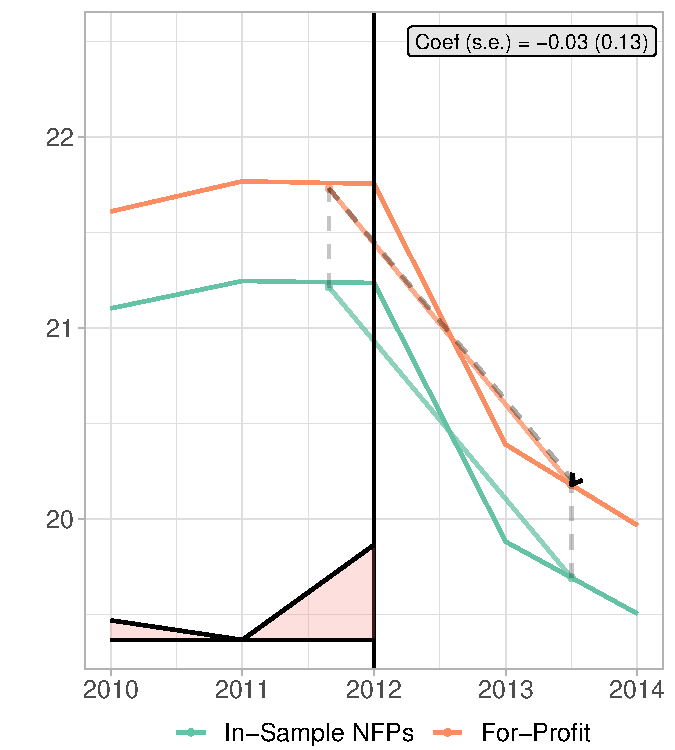
\includegraphics[width=\textwidth]{Objects/read_fp_nfp_synth_graph.pdf}
         \label{fig:read_synth_plota}
     \end{subfigure}%
     \hfill
     \begin{subfigure}[b]{0.45\textwidth}
         \centering
         \caption{For-Profit and NFP w/ MD Exec}
         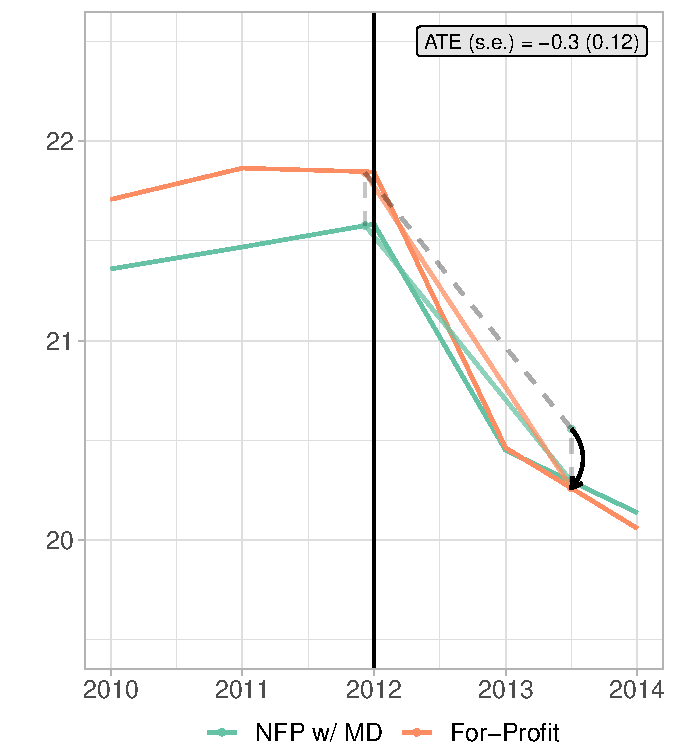
\includegraphics[width=\textwidth]{Objects/read_fp_md_synth_graph.pdf}
         \label{fig:read_synth_plotb}
     \end{subfigure}%
     \vspace{5mm}
     \hfill
     \begin{subfigure}[b]{0.45\textwidth}
         \centering
         \caption{For-Profit and NFP w/out MD Exec}
         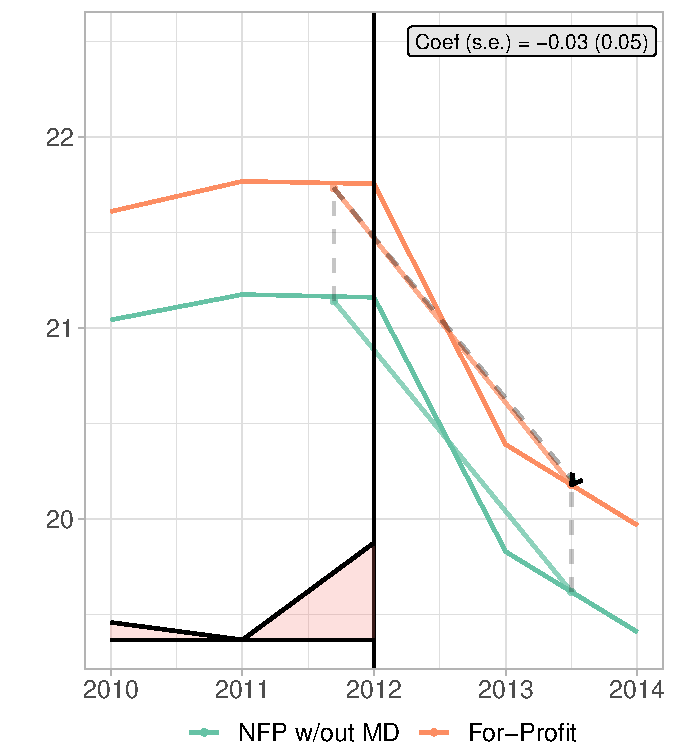
\includegraphics[width=\textwidth]{Objects/read_fp_nomd_synth_graph.pdf}
         \label{fig:read_synth_plotc}
     \end{subfigure}
     \hfill
     \begin{subfigure}[b]{0.45\textwidth}
         \centering
         \caption{NFP w/ and w/out MD Exec}
         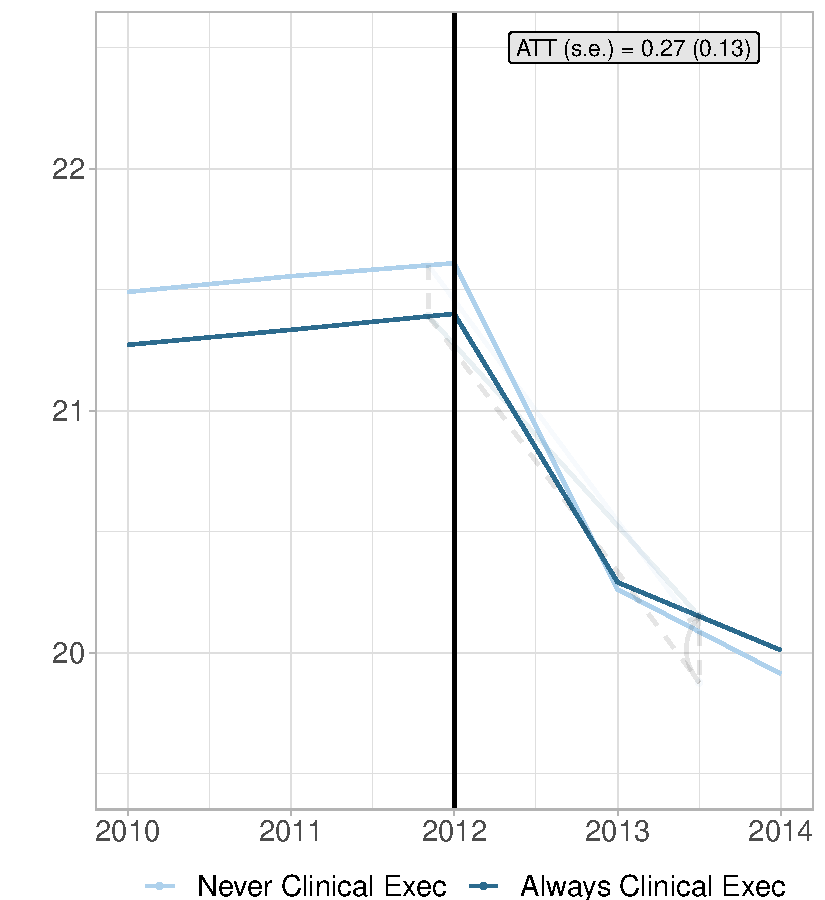
\includegraphics[width=\textwidth]{Objects/read_md_nomd_synth_graph.pdf}
         \label{fig:read_synth_plotd}
     \end{subfigure}
        \label{fig:read_synth_plot}
    \end{figure}

    Finally, in Figure \ref{fig:read_synth_plotd}, I present estimates of Equation \ref{eq:clinical}, directly comparing NFPs with and without clinical executives. NFPs without a clinically trained executive lowered readmission rates by .3ppts more than NFPs with a clinically trained executive. Relative to the average readmission rates in 2010, this is approximately a 1.5\% decrease, or 11 less readmissions per year. 

    Next, I present estimated differences in mortality rates between different hospital types in Figure \ref{fig:mort_synth_plot}. Figure \ref{fig:mort_synth_plota} compares for-profit and all NFP mortality rates after the pay-for-performance incentives. These results show that there is no statistical difference in mortality rates between for-profits and not-for-profits after the programs. However, when considering NFPs with different leadership team compositions, shown in in Figures \ref{fig:mort_synth_plotb} and \ref{fig:mort_synth_plotc}, there seems to be a difference in behavior. While mortality rates are significantly more noisy than readmission rates, the coefficient on the difference in mortality rates for for-profit compared to NFP with an MD is -.17, a magnitude similar to that of readmission rates. However, for-profits and NFPs without a clinical executive behave similarly. 

    I also directly estimate the difference in mortality rates among NFPs with and without clinical experience in Figure \ref{fig:mort_synth_plotd}. Again, the difference is not statistically significant, but this is likely due to the noisiness in mortality since the results is similar to that of readmission rates. NFP hospital without a clinically trained executive decrease mortality rates more than NFPs without a clinically trained executive due to new pay-for-performance incentives.

     \begin{figure}
     \caption{Mortality Rate Synthetic Difference in Differences Results}
     \centering
          \begin{subfigure}[b]{0.45\textwidth}
         \centering
         \caption{For-Profit and All NFP}
         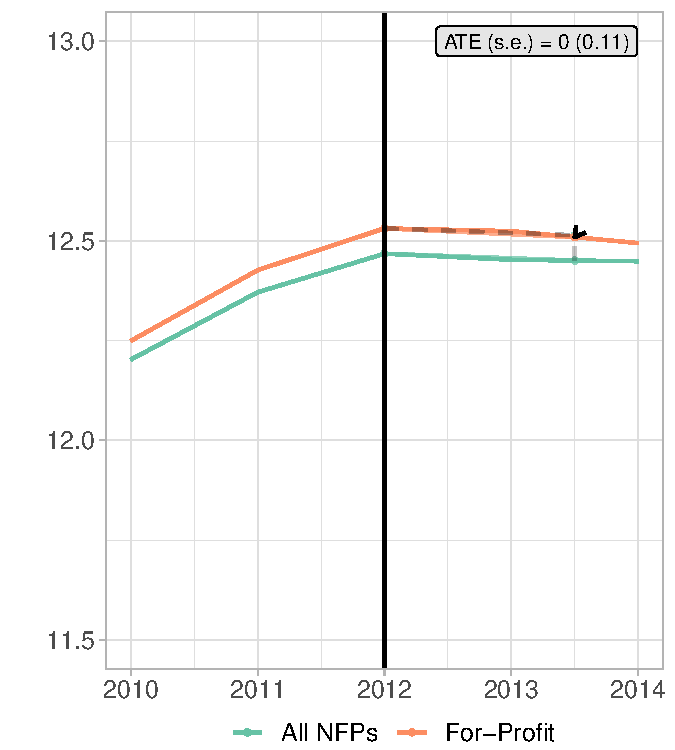
\includegraphics[width=\textwidth]{Objects/mort_fp_nfp_synth_graph.pdf}
         \label{fig:mort_synth_plota}
     \end{subfigure}%
     \hfill
     \begin{subfigure}[b]{0.45\textwidth}
         \centering
         \caption{For-Profit and NFP w/ MD Exec}
         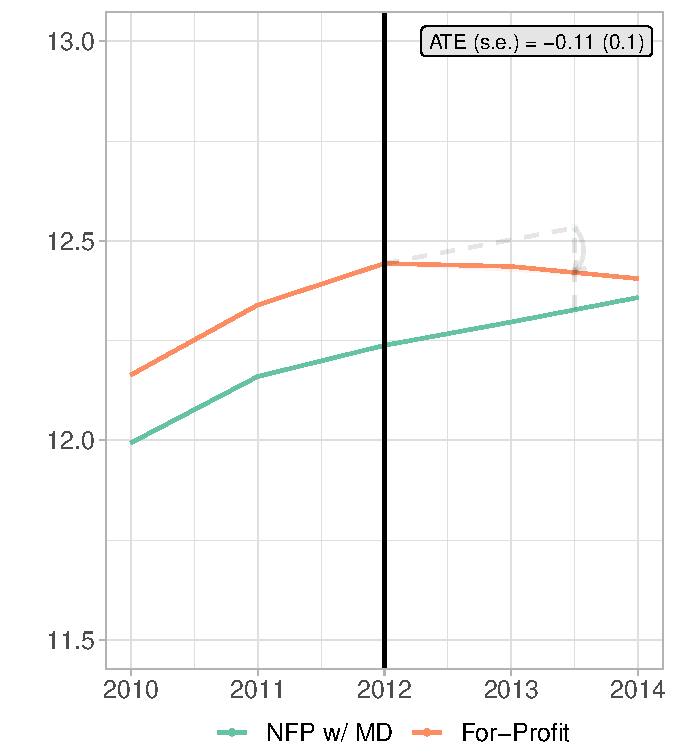
\includegraphics[width=\textwidth]{Objects/mort_fp_md_synth_graph.pdf}
         \label{fig:mort_synth_plotb}
     \end{subfigure}%
     \hfill
     \begin{subfigure}[b]{0.45\textwidth}
         \centering
         \caption{For-Profit and NFP w/out MD Exec}
         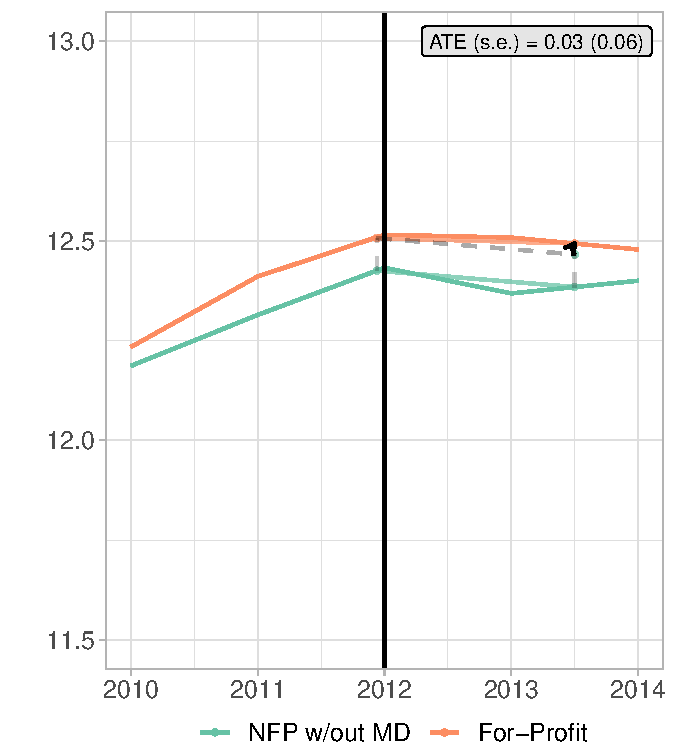
\includegraphics[width=\textwidth]{Objects/mort_fp_nomd_synth_graph.pdf}
         \label{fig:mort_synth_plotc}
     \end{subfigure}
     \hfill
     \begin{subfigure}[b]{0.45\textwidth}
         \centering
         \caption{NFP w/ and w/out MD Exec}
         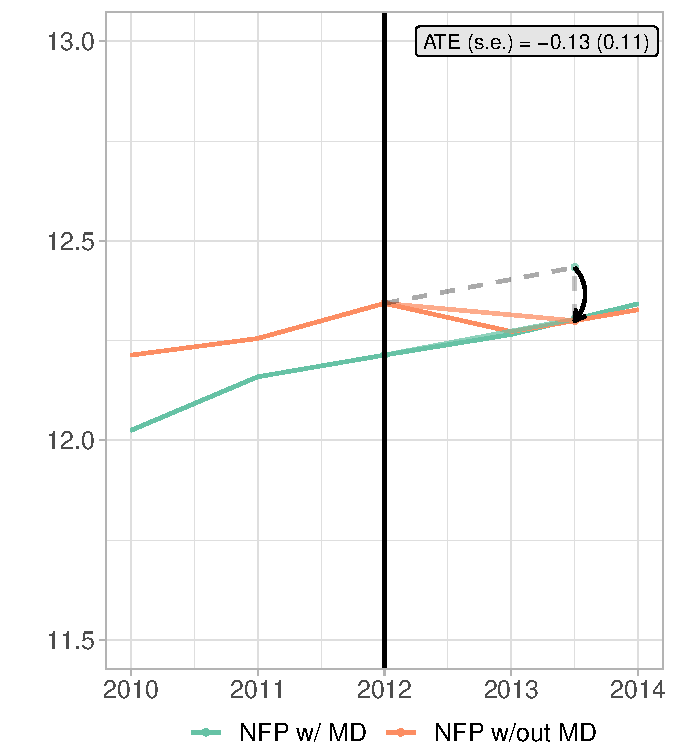
\includegraphics[width=\textwidth]{Objects/mort_md_nomd_synth_graph.pdf}
         \label{fig:mort_synth_plotd}
     \end{subfigure}
        \label{fig:mort_synth_plot}
    \end{figure}

    \subsection{Decomposition}

    While it is telling that executive team composition affects behavior after incentives change, more clarity is needed about the root cause of the differences. It is not clear whether these results are due to clinically trained executives being a signal of underlying hospital objectives, or the leaders themselves making a difference in outcomes. Therefore, I present the results of specification \ref{eq:decomp} in Table \ref{tab:MD_noMD_readmort_decomp_synth}, where the variation in executives is either existence of a hospital executive at any point in time, or whether the hospital has a clinically trained executive in 2012 when the programs were enacted. The left panel on readmission rates shows that the difference in response is fully driven by having a clinically trained executive in 2012 compared to having a clinically trained executive at another point in time. The right panel shows similar magnitudes of coefficients with more noise, as in the main specification.  

    \import{Tables}{MD_noMD_readmort_decomp_synth.tex}

     
 

    \section{Conclusion}

    In this paper, I study differential objective between different firm types. While the differences in for-profit and not-for-profit hospitals have been studied in the past, it is unclear whether certain not-for-profit characteristics make them act more like for-profits. In order to better understand the role of leadership in objectives, I estimate the differential response to a change in incentives among for-profits, not-for-profits, and not-for-profits with and without a clinically trained executive executives. I find that not-for-profits without clinically trained executives respond to incentives much more similarly to for-profits than to not-for-profits without clinically trained executives.

	
	\newpage

    \printbibliography

\appendix

 \section{Data}\label{appendixdata}

\subsection{Gathering Hospital Leadership Names}

There is no perfect way to access tax form 990s in bulk over the time period I am considering in this paper. However, using the not-for-profit Explorer API seems to be the most straightforward. At the time of writing this, information on using version 2 of the API can be found at \hyperlink{https://projects.propublica.org/not-for-profits/api}{https://projects.propublica.org/not-for-profits/api}. 
    
There are over 1.5 million not-for-profit entities in the US (cite), making it crucially important to be able to filter by type of entity before analyzing any PDFs. The API allows this by filtering a query based on National Taxonomy of Exempt Entities (NTEE) code. I query only not-for-profits categorized as E20 (hospitals), E21 (community health systems), and E22 (general hospitals). The API has a pagination limit of 100, meaning I can only pull information on 100 hospitals at a time. Therefore, I filter the query further to only consider one state at a time. The only state that has more than 100 entities registered is California, and thus I subset the California query even further by names that include the word "hospital" and names that don't. I combine all of these subsets and have information on each not-for-profits Employee Identification Number. There are 5,588 EINs total in this list. This acts as a list of entities for which I can pull more information. 

I loop through the list of EINs found in the previous step and query more detailed information from the API on that specific EIN. I save the name, secondary name, state, and zip code, all of which do not vary by year. I also save each year's URL that links to the Tax Form 990 PDF. For the sake of a comprehensive data set, I keep years 2006-2020 (I later limit to 2009-2016 when focusing on the Hospital Readmissions Reduction Program). Thus, I finish this step with a panel data set of EIN characteristics and PDF locations. Importantly, there are multiple types of Tax Form 990s depending on the size of the not-for-profit. In many cases, one not-for-profit has at least two different forms filed in a given year. I filter out any EIN-years for which there are no PDFs on file. The data on PDF locations contains 4,012 EINs and 61,363 EIN-year-tax forms.

It is crucial to the analysis to be able to link these not-for-profits with other sources of data to recover penalties from HRRP, bed size, and outcomes of interest (definitely need to talk more about outcomes). Therefore, I take a conservative approach to matching EINs to American Hospital Association (AHA) ID, which links fairly easily to Medicare ID numbers, based on name and location. First, I will discuss limitations and cleaning that I do to the AHA data and tax form data separately before doing any matching. 

I download the AHA data from Wharton Research Data Services. I filter only to hospitals in the contiguous US, Alaska, and Hawaii (excluding places like Puerto Rico), classified as not-for-profit or state/community, and those that are general acute care. I also filter out any hospitals who weren't present in the data (or change system ID) in 2009-2015, meaning they either closed or were acquired. Due to the survey nature of this data, a hospital name may look slightly different from one year to the next. For example, "Waldo County General Hospital" is also Waldo County General Hospital Maine Health". Further, zip codes may change by one or two digits, making them unreliable to match based on. To deal with this, I first keep only unique AHA ID, name, zip, state, and system name combinations. Then, I convert the data from long to wide so that each AHA ID occurs only once, but may have multiple names, zip codes, or system names associated with it.

I consider which not-for-profit entities are not likely to be hospitals and drop them. There are numerous foundations or auxiliary not-for-profits with the purpose of raising funds for the hospital, but do not actually care for patient. I filter out any not-for-profit with "foundation" or "auxiliary" in the name. I also filter out various specialty centers that fell into the general hospital category, such as hospice or cancer centers. 

I then proceed matching based on names in multiple layers. I focus on exact string matches, so I remove all spaces and common characters that could cause mismatches such as \&, ', -, and inc. Next, I take each AHA name and look for exact matches in a not-for-profit's first or secondary name only for not-for-profits in the same state as the AHA hospital. When an exact match is found, I record the link between AHA ID and EIN. In this first layer of matching, 860 hospitals in the AHA data are linked to an EIN, equivalent to 31\% of AHA not-for-profit hospitals in the sample. 

In the next layer of matching, I remove common words such as "healthcare", "regional", "hospital", etc. That way if there are subtle differences in names, removing common words may allow for an exact match. Again, I take each AHA hospital name and look for exact matches in the not-for-profits within the same state. This adds an additional 90 hospital matches, accounting for a total of 34.5\% of AHA hospitals. 

In some cases, tax forms are associated with a system of hospitals instead of one individual hospital. Thus, I create another variable that captures the names of systems which match. The process of matching is the same, the only difference is that now I am considering system names from the AHA data instead of hospital names. A total of 1,136 AHA hospitals have an EIN match on hospital name, system name, or both. This is roughly 41\% of the sample. These hospitals become the main sample for my analysis. While not capturing a large majority of AHA hospitals that are categorized as not-for-profit, I would rather be conservative in selecting hospitals which I am confident that the characteristics and measurement of the independent and dependent variables are accurate. 

(add a paragraph about validity of matches)

 Now that I have a sample of hospitals, the next step is to extract the names of the people in charge of these hospitals from the Tax Form 990 PDFs. In the data set of hospital PDF URLs that I collected earlier, I limit to the hospitals with solid matches described above. I then loop through each EIN, downloading each PDF locally and using tesseract package in R to extract text from the relevant pages of the PDF using OCR text extraction methods. In particular, I loop through each page of the PDF, look for the title associated with leadership names: ``Officers, Directors, Trustees, Key Employees, and Highest Compensated Employees", and save all the text from any pages where this title is found. I save the text to a list of all EIN, years present. 

One tricky aspect of the not-for-profit Explorer API is that, only in some cases, if two forms are present for an EIN, year, only the first one (which is typically not the one with the relevant information) is pulled. Therefore, for some hospitals, a couple years will have gaps in text extraction data. I locate EIN, years where this problem is occurring, and a team of RAs locates and downloads the correct forms manually. I extract text from these manually downloaded forms in the same manner as above. 

The form of the text data is a data frame with one column, where each line of text is saved in a different row. I write a text cleaning package that locates names, positions, titles, and indications of resigning. I will now describe this function in three parts: preliminary cleaning of strings, locating names, and locating positions, titles, and key words surrounding resigning. 

Typically on the same page as the names and positions is a list of the highest compensated employees and their compensation. In order to not record extra names, I filter out any rows after the start of this section. I then remove any digits, parentheses and brackets, other punctuation, letters that occur by themselves, two letter ``words" that have no meaning, and excess space between words. I then split up the phrase into individual words, so one phrase with 5 words is broken up into 5 variables. 

Next, I locate first and last names in the data. 

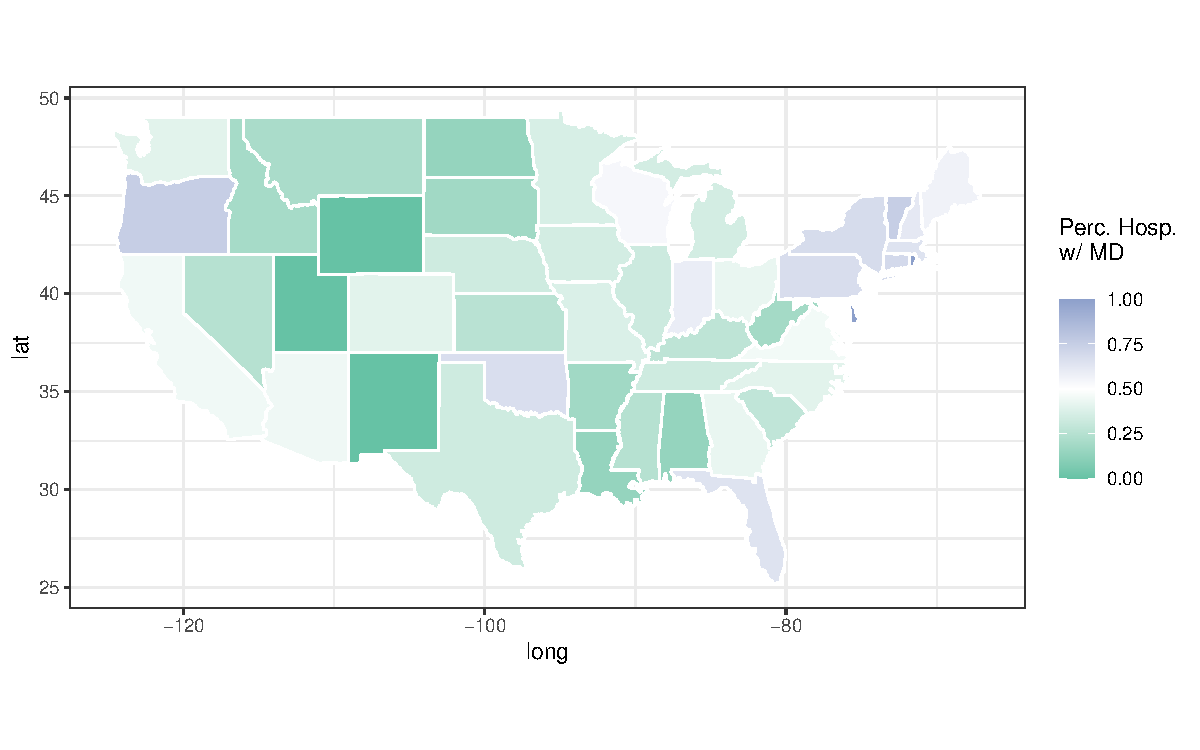
\includegraphics[width=\textwidth]{Objects/has_doc_avg_map.pdf}


\section{Hospitals Matched to AHA vs. Not}\label{app:matched}

\import{Tables}{NFP_sample_comparison.tex}

\section{Full Sample Regression and Event Study Results}\label{app:fullsample}

\import{Tables}{MD_noMD_readmort_fullsample.tex}

\import{Tables}{forprofit_readmort_fullsample.tex}

\import{Tables}{MD_noMD_uncompCMI_fullsample.tex}

\import{Tables}{forprofit_uncompCMI_fullsample.tex}

\section{Synthetic Diff-in-Diff Result Tables}

\import{Tables}{forprofit_readmort_synth.tex}

\import{Tables}{MD_noMD_readmort_synth.tex}


    

    

    

    

    

    

	
	
	


\end{document}

